\chapter{Experiment}
\section{Plasma Spray-PVD}
\subsection{PS-PVD apparatus}
To produce the Si:Ni nanoparticle, the hybrid plasma with two torch(DC and RF) is used.
\begin{figure}[h]
\centering
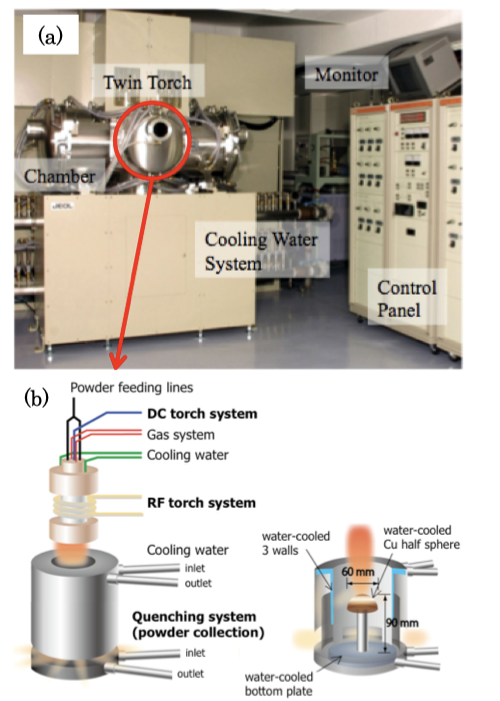
\includegraphics[width=8cm]{src/fig/fig20.png}
\caption{(a)PS-PVD apparatus; (b)illustration of a plasma generator and water-cooling system}
\end{figure}
In the upper part of apparatus, there are two DC torches available for plasma spray process, and here only one torch is used for our research. The maximum DC power is 15 kW and maximum RF power is 150 kW. The chamber is evacuated by a PID pressure controller with a 1200 L/s mechanical booster pump and two 2500 L/s water seal pumps. The pressure can be reduced up to 1 Pa. The detailed condition is described in table 2.1.\\
\begin{figure}[h]
\centering
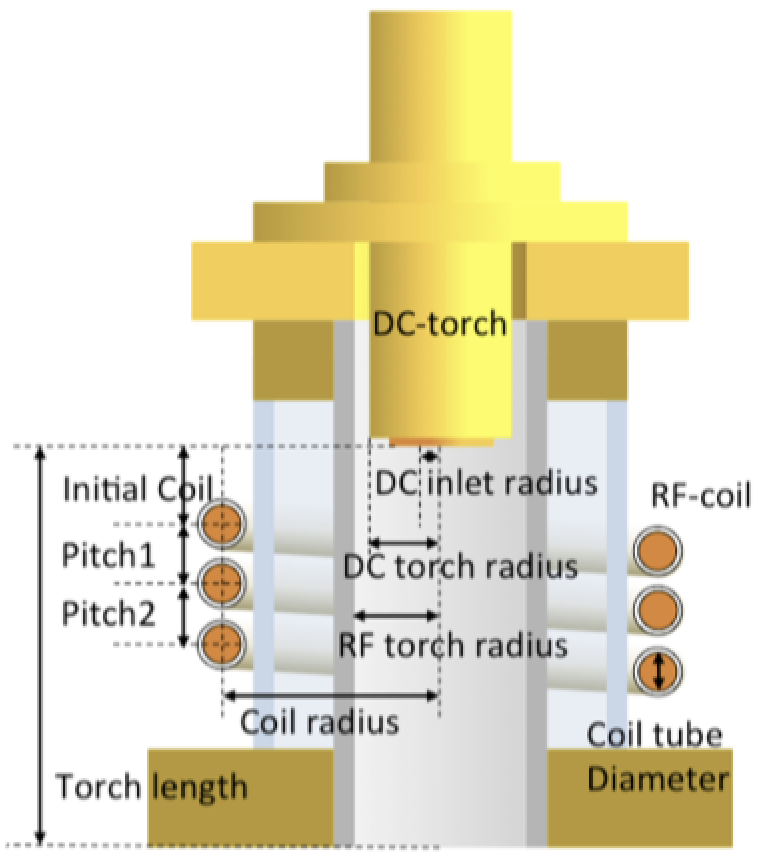
\includegraphics[width=8cm]{src/fig/fig21.png}
\caption{The schematic illusion of a hybrid torch}
\end{figure}

\begin{table}[htbp]
\centering
\caption{ Torch condition}
\begin{tabular}{cc}
\toprule
Parameter & Value\\
\midrule
DC inlet radius(mm) & 4 \\
DC torch radius(mm) & 20 \\
RF torch radius(mm) & 21 \\
Coil tube diameter(mm) & 8 \\
Initial coil(mm) & 22 \\
Pitch 1(mm) & 21.5 \\
Pitch 2(mm) & 21.5 \\
Torch length(mm) & 98 \\
Coil radius(mm) & 33.5 \\
\bottomrule
\end{tabular}
\end{table}

Metallurgical Si(MG-Si) powder is used as a raw material. Unlike Semiconductor Grade Silicon (SEG-Si) or Solar Grade Silicon(SOG-Si), MG-Si allows impurities(98\%~99\%), so it is much cheaper. The average size of MG-Si particle is 19.2 µm as measured by the laser diffraction / scattering method. The powder feeder used is TWIN 10C POWDER FEEDER from SULZER METECO company. The carrier gas is Ar, introduced radially and tangentially, and the flow rate is set to 3.6 slm. A predetermined amount of Ni powder and Si powder mixture is injected to plasma, they are evaporated and co-condensed on the copper plate at the bottom of reactor. 
\subsection{PS-PVD condition}
\begin{table}[H]
\centering
\caption{PS-PVD condition}
\begin{tabular}{cc}
\toprule
Parameter & Value\\
\midrule
Torch diameter(mm) & 60 \\
Torch length(mm) & 150 \\
DC power(kW) & 8 \\
RF power(kW) & 90 \\
DC Ar(slm) & 10 \\
Tangential Ar(slm) & 140 \\
Radial Ar(slm) & 30 \\
Ni addition(at.\%) & 0,5 \\
Powder feeding rate(g/min) & 1 \\
Chamber pressure(torr) & 400 \\
\bottomrule
\end{tabular}
\end{table}
\section{Plasma Enhanced-CVD}
\subsection{PE-CVD apparatus}
\begin{figure}[H]
\centering
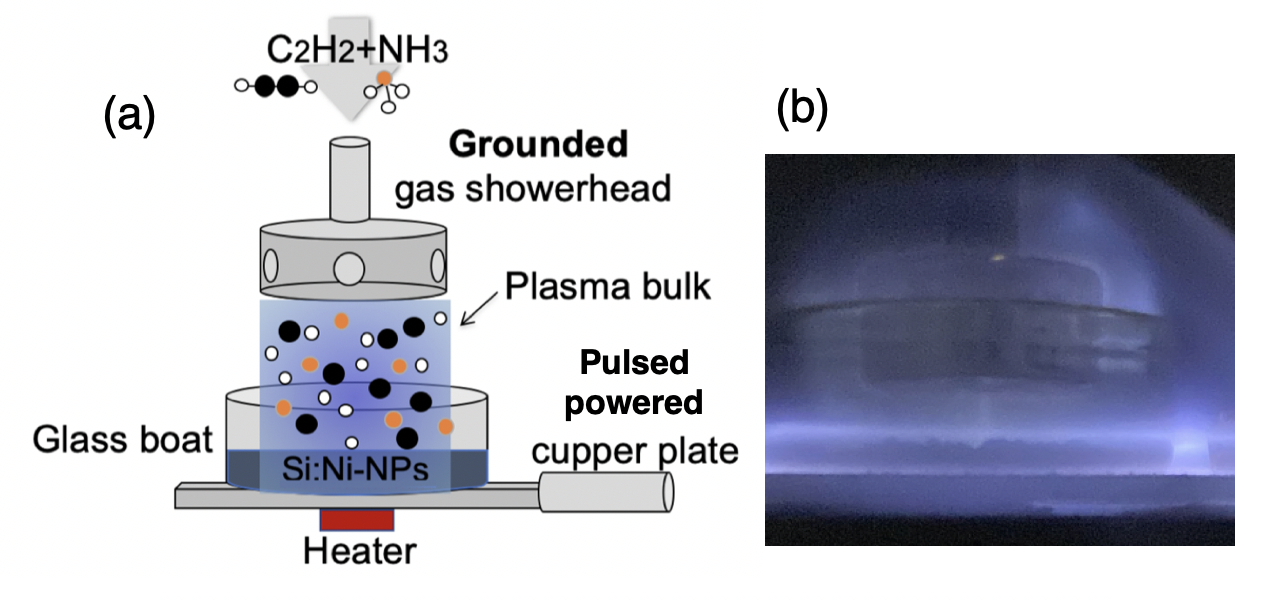
\includegraphics[width=14cm]{src/fig/fig22.png}
\caption{(a)The generation of plasma in PE-CVD.(b)The illustration of Plasma-enhanced CVD.}
\end{figure}
The $\mathrm{C_{2}H_{2}}$ is used as carbon source and $\mathrm{NH_{3}}$ as the dilute gas. The glass boat with a diameter of 3 cm loads the Si:Ni-NP powders and the heater is fixed beneath the copper plate. The power unit to generate plasma is PVM400/DELUX adjustable power supply, of which the output varies from 1 to 20 kV, the frequency varies from 20 to 60kHz and current is up to 25 mA. The micro ceramic heater is MS-1000-10 series from SAKAGUCHI Corp. The maximum temperature of the heater surface can attain 1000\(^\circ\)C at maximum voltage. However, due to the heat dissipation, the actual temperature of copper plate is much lower (350\(^\circ\)C). Initially, we adopted the typical plasma generation method where the gas shower head is grounded and the copper plate is powered. However, once apply RF power on gas shower head , Si:Ni-NP powders exploded due to the discharge. Then we modified the set-up, reversed the electrodes to make it a dielectric-barrier discharge (DBD), with insulating glass boat being the barrier. Finally the explosion problem is solved.There are several parameters that can be controlled to investigate the optimal CNT growth condition: pressure, annealing time, plasma power, flow rate of reacting gases and temperature.

\subsection{CNT growth condition}
\begin{table}[H]
\centering
\caption{Parameters in PE-CVD}
\begin{tabular}{cccc}
\toprule
Parameter          & \multicolumn{3}{c}{Value}                     \\
\midrule
Temperature(\(^\circ\)C)        & 100            & 200           & 300          \\
Pressure(torr)           & \multicolumn{3}{c}{2}                         \\
Electrode distance(cm) & \multicolumn{3}{c}{1}                         \\
Plasma power       & \multicolumn{3}{c}{1$\sim$20kV,20$\sim$60kHz} \\
$\mathrm{C_{2}H_{2}:NH_{3}}$ flow rate(sccm)           & 14:70          & 14:35         & 14:14        \\
Annealing time(min)     & \multicolumn{3}{c}{15}    \\                 \bottomrule  
\end{tabular}
\end{table}

\newpage

\section{Battery assembly}
\begin{figure}[H]
\centering
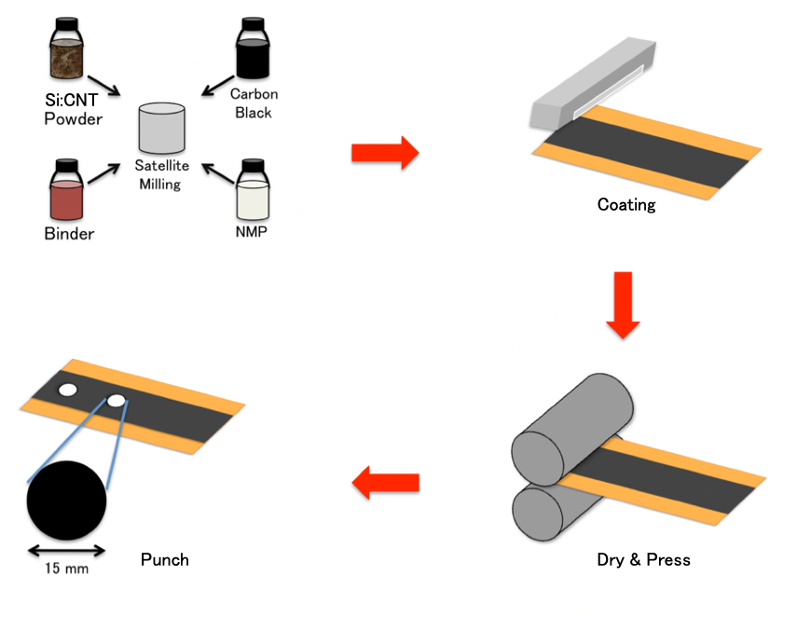
\includegraphics[width=10cm]{src/fig/fig23.png}
\caption{The procedure of battery assembly}
\end{figure}
As shown in Fig. 2.4, the assembly of of a battery can be divided into four steps: slurry preparation, coating, drying and pressing, punching.
\subsubsection{Slurry and milling}
The PS-PVD and PE-CVD processed particles act as the active material in an anode. The particles are sieved to be smaller than 45 um. Then mix with the polyimide binder(25\%), the N-methylpyrrolidone (NMP) solvant (3.3$\sim$4.4 times of the weight of active materials) and carbon black(15\%) in a zirconia container. To well mix them, three zirconia balls with a diameter of 5 mm are put in the container. The container is then centrifuged at 800 rpm for 5 minutes in a centrifuge to produce a slurry. The polyimide binder adheres the active material to the current collector, and the carbon black is conductive material that enhanced the overall conductivity of full cell. NMP was used to adjust the viscosity of the slurry so that the slurry could be applied evenly.
\subsubsection{Coating}
The slurry was applied onto a 12 µm copper foil using a doctor blade for a primary thickness of 75 µm.
\subsubsection{Dry and press}
The slurry on copper foil was then air dried at 110 \(^\circ\)C in an oven, for 15 minutes. In order to improve the adhesiveness and gain uniform thickness, this slurry on copper foil is pressed at 10 kN and dried for another 45 minutes.
\subsubsection{Punch}
The dried slurry is punched into a circle with a diameter of 15 mm so that fits into the coin cell. The mass measured five times and thickness are measured twice.
Figure 2.5 shows the components of a typical half cell. The assembly is operated in a globe box with an inert Ar atmosphere to prevent oxidation of electrodes. The Metal Li is used for the opposite electrode of the half cell. The solvent is Ethylene carbonate and diethyl carbonate with a 1:1 (v:v) ratio. LiPF6 is used as the electrolyte, and a polyolefin porous film is used as the separator. After placing them at the certain sequence, the coin cell case with a rubber gasket is punched by a caulking machine.
\begin{figure}[H]
\centering
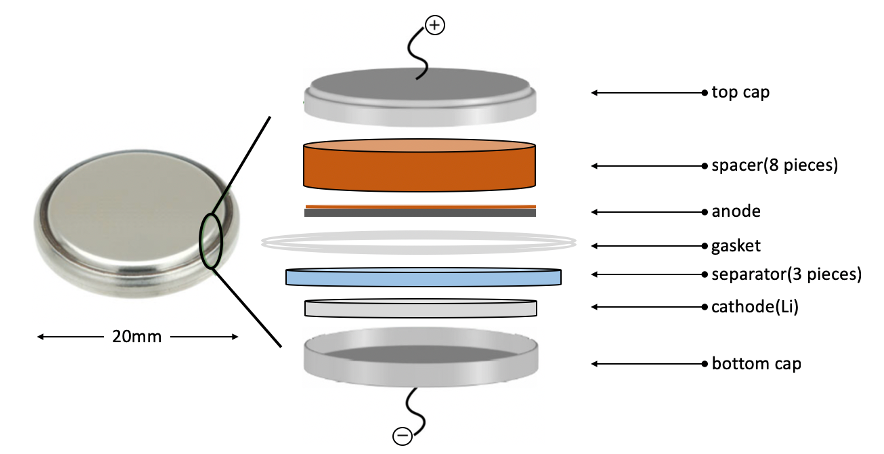
\includegraphics[width=10cm]{src/fig/fig24.png}
\caption{Configuration of  a half cell}
\end{figure}
\section{Powder characteristics}
\subsection{X-ray diffraction (XRD)\textsuperscript{[24]}}
The X-ray diffraction (XRD) was used to determine the crystallographic structure of the phases present and to determine if any preferred orientation (or texture) was present in the materials. If the powder is placed in the path of a with specific X-ray beam of a constant wavelength $\lambda$, Rayleigh scattering occurs and certain diffraction will occur from the planes in those crystallites that are oriented at the correct angle to fulfill the Bragg law.
The Bragg law is,
$$n\lambda=2dsin\theta$$
$d$ is the inter planar spacing of a crystal, $n$(an integer) is the order of reflection, and $\theta$ is the diffraction incident angles.
\begin{figure}[H]
\centering
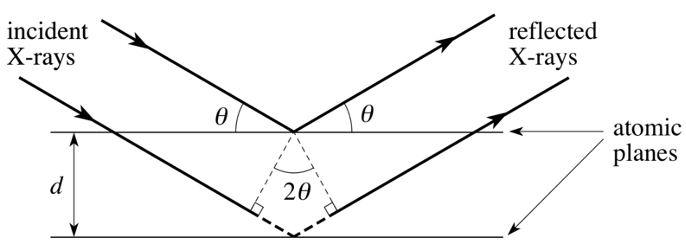
\includegraphics[width=8cm]{src/fig/fig25.png}
\caption{The reflection of Bragg's Law\textsuperscript{[24]} }
\end{figure}
The basic configuration of XRD consists of an X-ray generator, an X-ray filter, a goniometer, a detector, a pulse height analyzer, and a counting circuit. The X-ray generator consists of an X-ray tube class for generating primary X-rays and a power supply that applies a high voltage. The thermions from the tungsten filament kept at a high negative potential are accelerated and collide with the negative electrodes such as Cu, Fe, and Co to emit their characteristic X-rays ($K_\alpha$).  
In this experiment, the $\mathrm{D_{2}}$ PHASER (Bruker Corp.) instrument was
used. Figure 2.11 is a configuration  of X-ray diffraction measurement. A piece of sample is placed in the center of the goniometer. By moving the shutter ,the constantly running X-rays reaches the sample in a specific angle. The sample holder  rotate at certain speed so the to adjust the incident X-ray for diffraction. 
\begin{figure}[H]
\centering
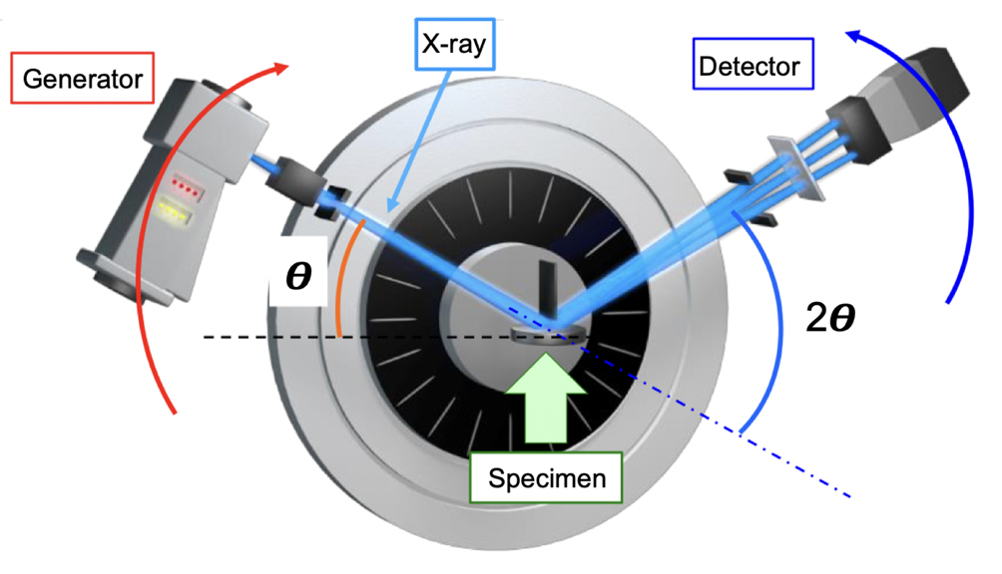
\includegraphics[width=8cm]{src/fig/fig26.png}
\caption{The configuration of XRD instrument\textsuperscript{[25]}}
\end{figure}

\begin{table}[H]
\centering
\caption{XRD condition}
\begin{tabular}{cc}
\toprule
Parameter              & Value                                        \\
\midrule
X ray generating power & 30 kV - 10 mA                                  \\
DS                     & 1 mm                                          \\
Primary solar slit     & $2.5^{\circ}$                                         \\
Secondary solar slit   & $2.5^{\circ}$                                         \\
Diffraction method     & $\mathrm{2\theta /\theta}$  \\
Step size              & $0.02^{\circ}$                                        \\
Scan speed             & 1.0 sec/step    \\                      \bottomrule      
\end{tabular}
\end{table}
\subsubsection{Rietveld analysis\textsuperscript{[26][27]}}
Rietveld analysis is a technique that has been developed for solving/refining crystal structures from powder diffraction data. The method takes a trial structure, calculates a powder diffraction profile and compares it to the measured profile. The trial structure is modified by changing various refinable parameters, including atomic positions, thermal parameters, site occupancies, peak shape parameters, etc., until a best-fit match is obtained with the measured pattern.  Rietveld analysis is especially useful in  quantitative crystalline phase analysis. However, it presents difficulties in quantitative determination of the fraction of the material amorphous part. This way, quantitative percentage of crystalline phases, determined by Rietveld Method, are relative, not considering the amorphous phase, namely,  amorphous carbon in our case.

\subsection{Size distribution\textsuperscript{[28]}}
Laser diffraction is a widely used particle sizing technique for materials ranging from hundreds of nanometers up to several millimeters in size. The way for it to  measures particle size distributions is to measure the angular variation in intensity of light scattered as a laser beam passes through a dispersed particulate sample. It is known that large particles scatter light at small angles and small particles scatter light at large angles. The angular scattering intensity data is analyzed to calculate the size of the particles responsible for creating the scattering pattern, using the Mie theory of light scattering. The particle size is reported as a volume equivalent sphere diameter.

In this experiment, WINGSALD7100 device of  Shimadzu Corporation is employed for particle size distribution measuring. In the work, a highly monochromatic ultraviolet region laser ($\lambda$= 375 µm) generated from a semiconductor laser source is used, and after converting to a parallel beam with a collimator, the particle group is irradiated. The scattered light from this group of particles up to a wide angle of 60 ° is collected by the lens, and concentric diffracted / scattered circles are formed on the detection surface at the focal length. This image is detected by a detector (Wing sensor). In addition, not only the front but also the lateral and rear diffracted light are detected. The particle size distribution is then calculated based on Fraunhofer’s diffraction theory and Mie’s scattering theory.
\begin{figure}[h]
\centering
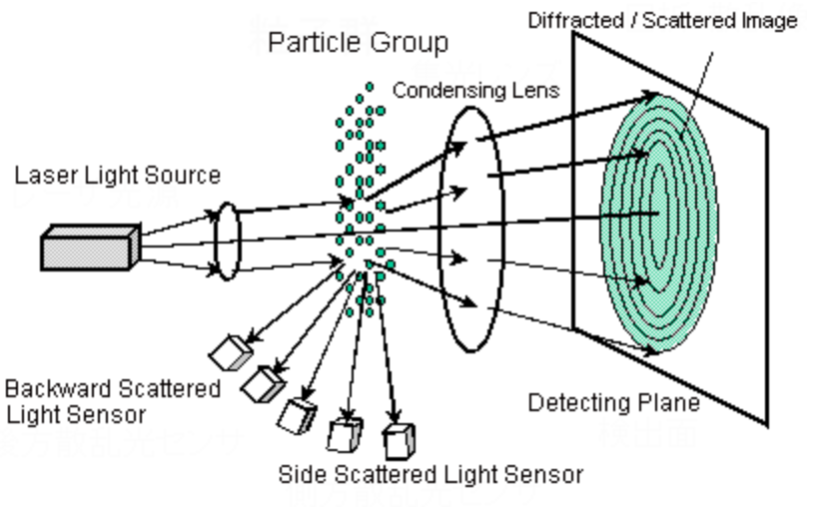
\includegraphics[width=8cm]{src/fig/fig27.png}
\caption{The configuration of laser diffraction system}
\end{figure}

\subsection{Scanning Electron Microscope(SEM)\textsuperscript{[29][30]}}
The Scanning Electron Microscope (SEM) is used for observation of specimen surfaces. When the specimen is irradiated with a fine electron beam (called an electron probe), secondary electrons are emitted from the specimen surface. Morphology of the sample surface can be observed by two-dimensional scanning of the electron probe over the surface and acquisition of an image from the detected secondary electrons. The SEM requires an electron optical system to produce an electron probe, a specimen stage to place the specimen, a secondary-electron detector to collect secondary electrons, an image display unit, and an operation system to perform various operations (Fig. 2.12). The electron optical system consists of an electron gun, a condenser lens and an objective lens to produce an electron probe, a scanning coil to scan the electron probe, and other components. This system (inside of the microscope column) and a space surrounding the specimen are kept in vacuum.
\begin{figure}[H]
\centering
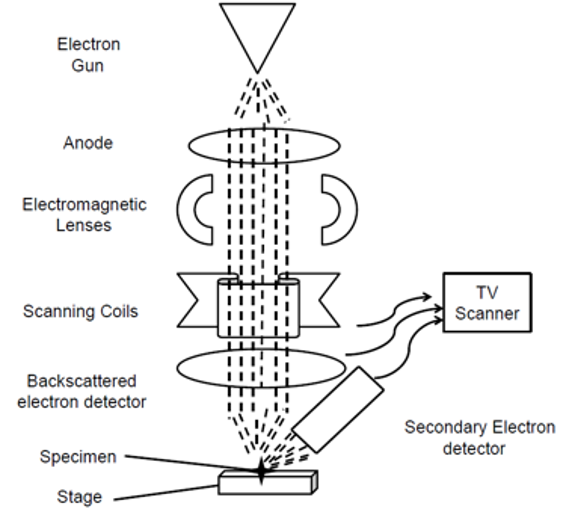
\includegraphics[width=8cm]{src/fig/fig28.png}
\caption{The electron optical system of SEM\textsuperscript{[28]}}
\end{figure}
In this experiment, S-4200 FIELD EMISSION SEM of HITACHI is used.
\subsubsection{Energy Dispersive Spectroscopy(EDS)\textsuperscript{[31]}}
The EDS is used to analyze characteristic X-ray spectra by measuring the energies of the X-rays. When the X-rays emitted from the specimen enter the semiconductor detector, electron-hole pairs are generated whose quantities correspond to the X-ray energy. Measuring these quantities (electric current) enables you to obtain the values of X-ray energy. The detector is cooled by liquid nitrogen, in order to reduce the electric noise. The advantage of the EDS is that the X-rays from a wide range of elements from B to U are analyzed simultaneously. 
\subsection{Raman Spectroscopy\textsuperscript{[32]}}
Raman is a light scattering technique, whereby a molecule scatters incident monochromatic light from a high intensity laser light source. Most of the elastic scattered light is at the same wavelength (or color) as the laser source and does not provide useful information – this is called Rayleigh Scatter. However a small amount of light (typically 0.0000001\%) is inelastic scattered at different wavelengths (or colors), the interaction between the phonons and the laser light results in a shift in energy, and this shift provides information about the modes of phonons in the system, namely, the rotational, vibrational, and other modes of a system.
\begin{figure}[H]
\centering
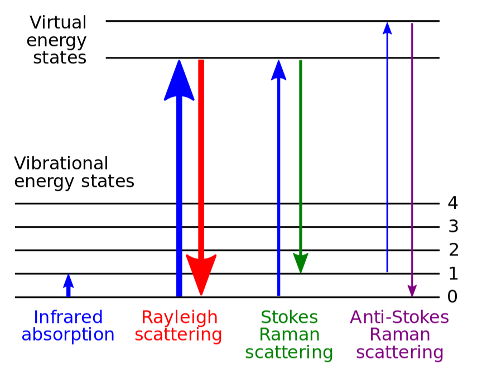
\includegraphics[width=8cm]{src/fig/fig29.png}
\caption{The energy-level diagram of  in Raman spectroscopy\textsuperscript{[33]}}
\end{figure}
If the emitted radiation is of lower frequency than the incident radiation, then it is called Stokes scattering.  If it is of higher frequency, then it is called anti-Stokes scattering. Though any Raman scattering is very low in intensity, the Stokes scattered radiation is more intense than the anti-Stokes scattered radiation. The reason for this is that very few molecules would exist in the excited level as compared to the ground state before the absorption of radiation. Information on the population of a phonon mode is given by the ratio of the Stokes and anti-Stokes intensity of the spontaneous Raman signal. 
\subsection{Transmission electron microscopy(TEM)\textsuperscript{[34]}}
Transmission electron microscopy (TEM) is the original form of electron microscopy and analogues to the optical microscope. It can achieve a resolution of ~0.1 nm, thousand times better resolution, cannot be reached by the light microscope. The beam of electrons passes through the specimen and analyzes the internal structure of the specimen in the form of images. The electron has the poor penetrating capability and gets absorbed in the thick specimen. Therefore, the thickness of the specimen should not be more than few hundred Angstroms ($10^{-10}$ m).  TEM provides information in the form of variations of electron intensity in the image. The electron image is monochromatic and must be made visible to the eye either by allowing the electrons to fall on a fluorescent screen fitted at the base of the microscope column or by capturing the image digitally for display on a computer monitor.
\begin{figure}[H]
\centering
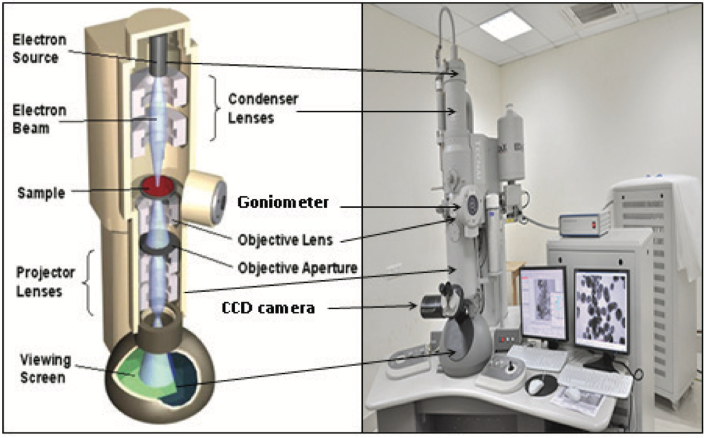
\includegraphics[width=8cm]{src/fig/fig30.png}
\caption{The electron beam system in TEM\textsuperscript{[34]}}
\end{figure}
In this research, the JEM-2010F (acceleration voltage = 200 kV, field emission gun, Tietz F416 camera) is used.
\subsection{Battery  test}
The impedance is an important factor that determines a LIB good or not.  The ex-situ impedance test is carried out with a frequency response analyzer (Solartron1260), an electrochemical interface (Solartron 1287). Set DC Potential as 0 (vs. Open Circuit) and AC amplitude as 10mV. The starting frequency is 1E-6 Hzand it ends at 0.1 Hz. The interval is set to be 10.  The impedance test is performed before charge/discharge service. The impedance is shown in Nyquist plot, in which the data from each frequency point is plotted by theimaginary part on the ordinate and the real part on the abscissa. There are many method to fit the Nyquist plot to do quantitative analysis of impedance. But In this research, qualitative analysis is done by comparing the radius of semicircle, which is enough to tell the good or bad conductivity of a half cell.

The capacity of a battery is expressed as the amount of electricity that can be taken out by discharging a battery charged under certain conditions under certain conditions and reaching the discharge end voltage, so it is affected by the charging / discharging method. Therefore, it is necessary to set appropriate charge / discharge conditions.

In this study, the ACD-01 charge / discharge tester manufactured by Asuka Electronics Co., Ltd. was used as the battery tester. In the battery test, charging and discharging were performed by the constant current method (CC) in which the cutoff voltage was set. Generally, the C rate is used to represent the charge / discharge current value. 1 C means the current value when the capacity of the battery is discharged in 1 hour. Similarly, 0.5 C discharges in 2 hours and 0.1 C discharges in 10 hours. This time, a charge / discharge test was conducted under the conditions of a cut-off voltage of 1.5 V to 0 V, 0.02 C for the initial 3 cycles, and 0.1 C for the 4th and subsequent cycles.

